\section{Dokumentstruktur - N+1}
N+1 modellen er anvendt, også kendt som 4+1 modellen. N+1 er bygget op så man kan se use casene på N forskellige måder. Figur \ref{fig:n+1} herunder giver viser de sektioner der er anvendt i dette projekt, normalt er der også en sektion der hedder Deployment view/Physical view, den er ikke inkluderet i dette projekt da der ikke er noget hardware\fxnote{lav dette om hvis vi vælger at bruge en i 4+1 alligevel. Det gælder også tegningen}.   

\begin{figure}[H]
	\centering
	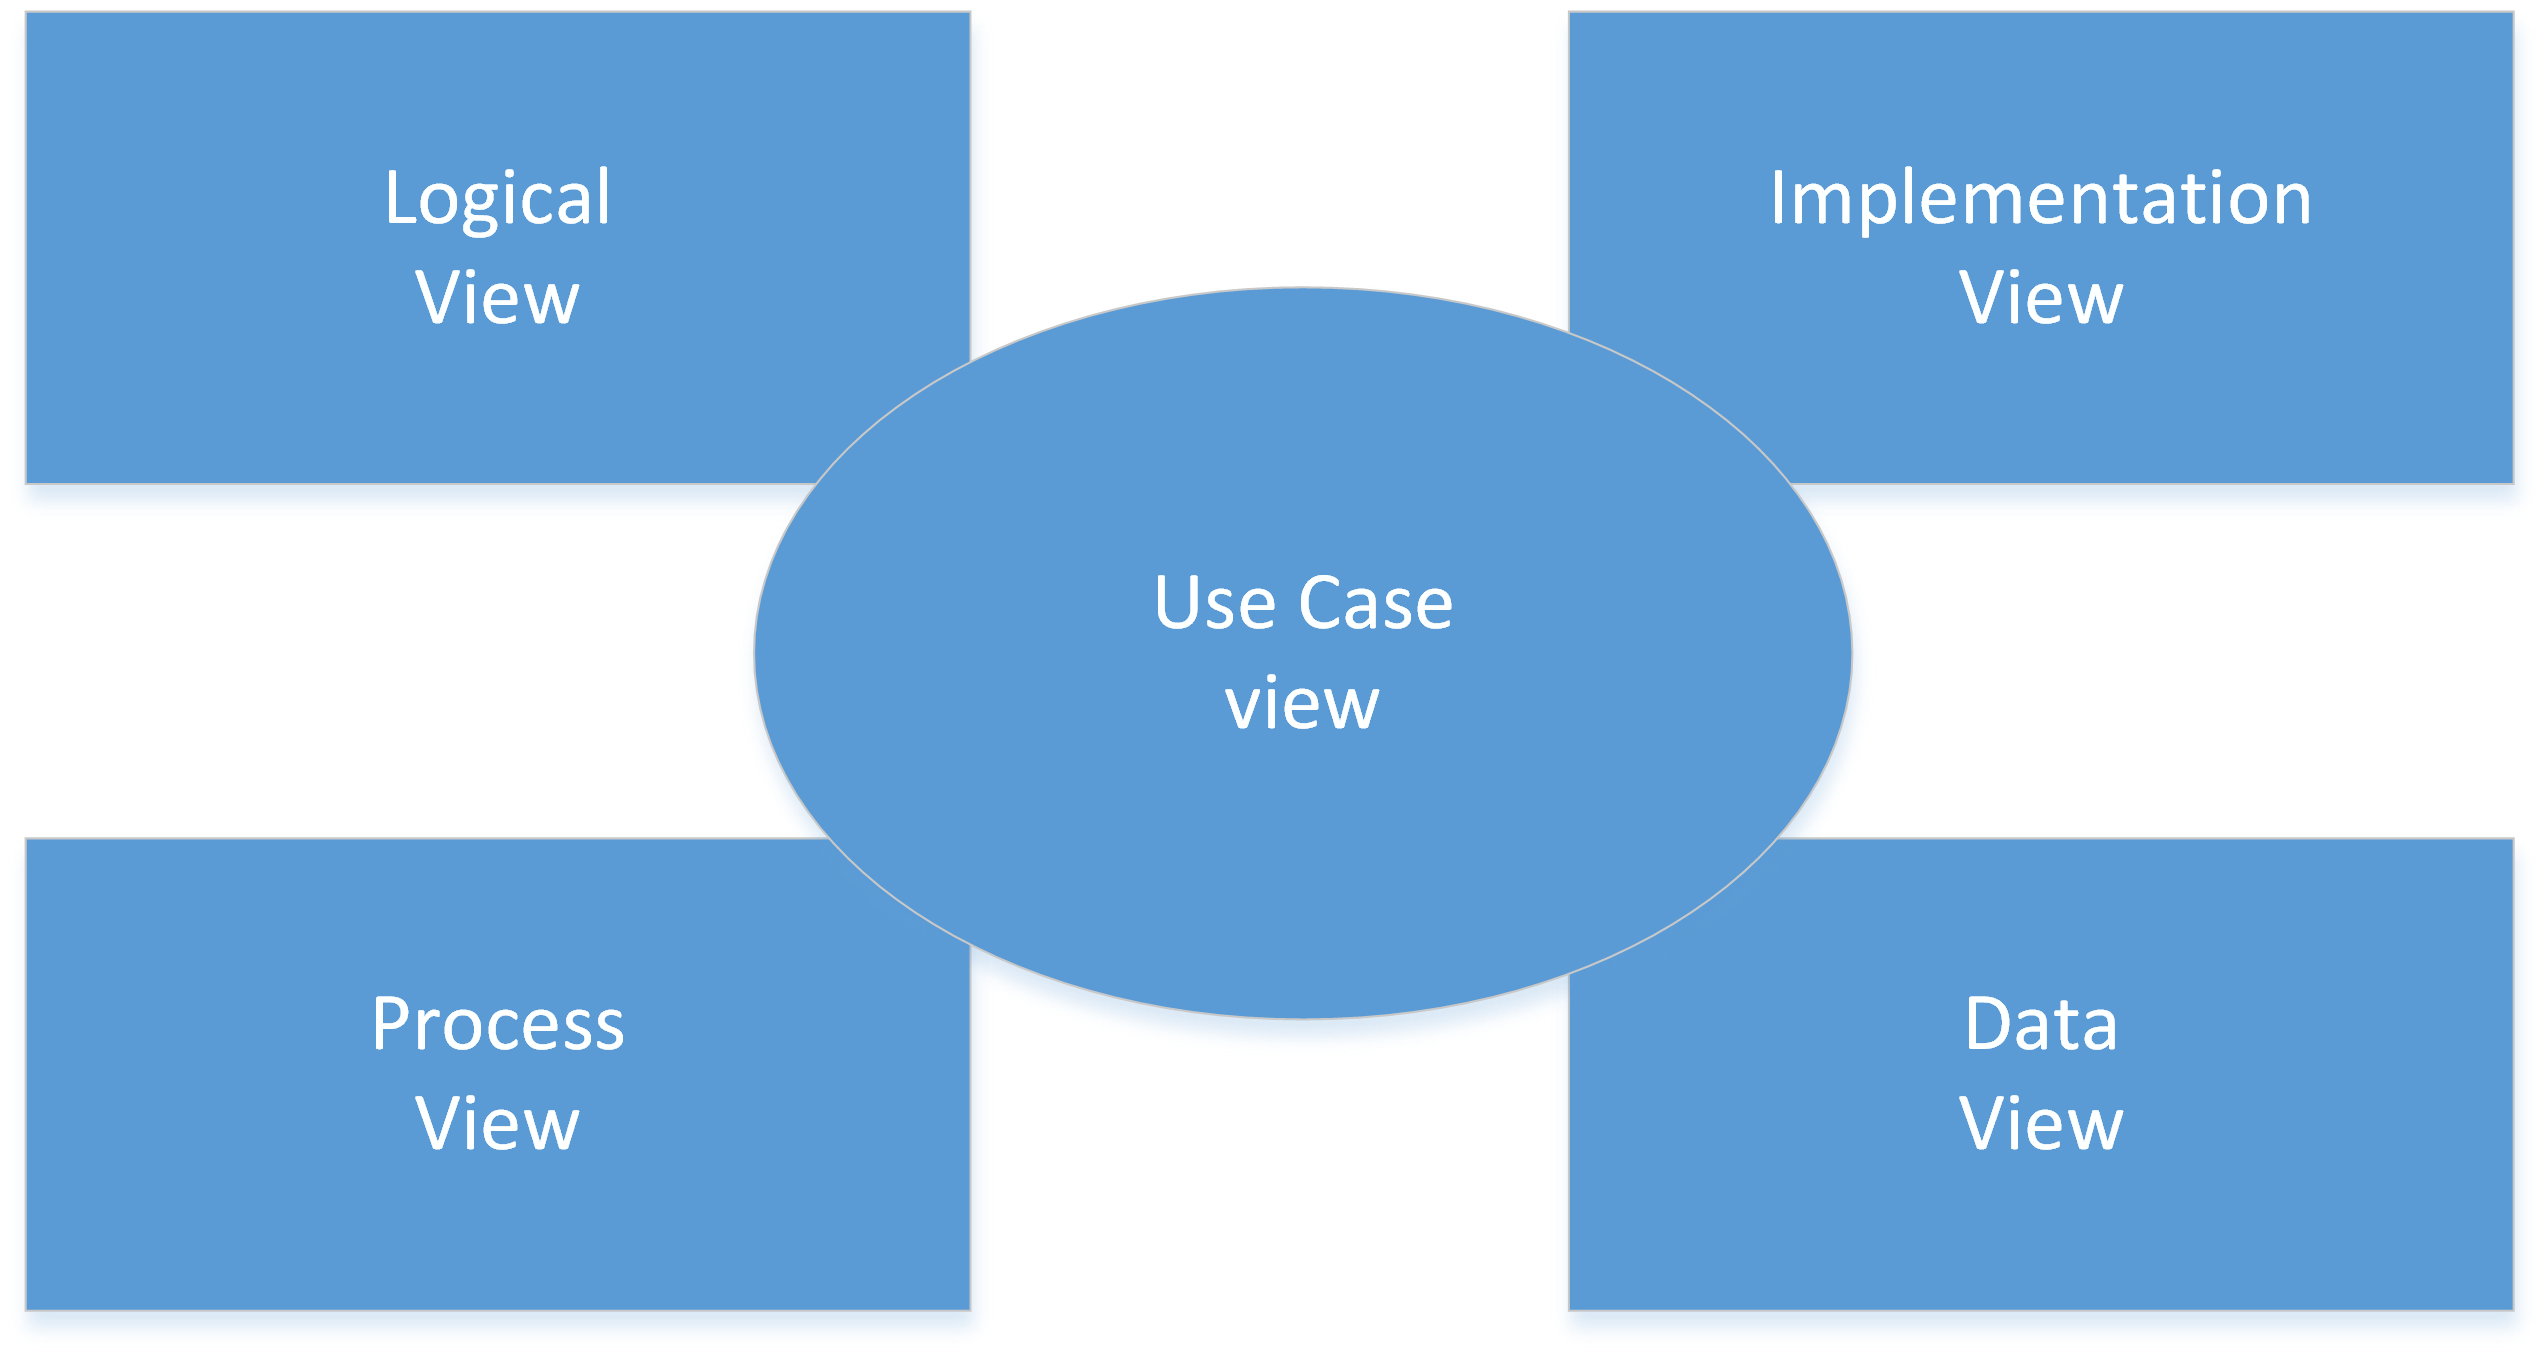
\includegraphics[width=0.8\textwidth]{N+1/N+1.png}
	\caption{N+1 modellen}
	\label{fig:n+1}
\end{figure}

\fxnote{beskrivelse af hvad der bliver gjort i de forskellige sektioner}

